\providecommand{\main}{..}
\documentclass[\main/main.tex]{subfiles}

\begin{document}
\graphicspath{{img/}{position_estimation/img/}}
\chapter{Position Estimation}

In this chapter, a position estimation technique is introduced. The ultimate aim of this technique is to be simple enough to run on a microcontroller while providing reasonable accuracy. Section \ref{sec:distance_measurement_using_time_of_flight} discusses about techniques used for distance measurement. A solution for solving location from distances to known points is proposed in chapter \ref{sec:localization_using_multilateration}. The final section, on the other hand, gives a method for converting the time of flights to actual distances used for positioning.

\section{Distance Measurement Using Time-of-Flight}
\label{sec:distance_measurement_using_time_of_flight}

\subsection{RSSI vs Time of Flight Distance Estimation}
There are two well-known methods to measure distances between two devices: using Received Signal Strength Indication (RSSI) and using Time of Flight (ToF).
\newline\newline
The RSSI method is based on the fact that the signal strength drops with increasing distance from the transmitter in a deterministic fashion following theoretic formulas. With this assumption, the distance between a receiver and transmitter can be estimated. This approach, however, has several disadvantages. Since the environment and the radio channel changes constantly, RSSI parameters are unstable, which in turn brings inaccuracy to the system. The multi-path propagation and other phenomena that are quite common for the radio channel can also degrade the accuracy. Traditional technologies like Wi-Fi, Bluetooth Low Energy are based on this distance estimation method.
\newline\newline
The second approach is to use the signal’s ToF rather than RSSI. This may yield much more accurate results in LoF (Line of Sight) environments and can lead up to a decimeter-level accuracy depending on the frequency and nature of the signal. An accurate position with a precision of up to several decimeters can be obtained by combining the ToF measurements from several devices. The performance might be degraded by obscuring the LoF between devices. Nevertheless, in comparison to the RSSI-based method, the overall accuracy is still superior. The ToF-based method is used by Ultra-Wideband technology. The nature of UWB signals makes it an ideal candidate for utilizing the ToF distance estimation process. 
\newline\newline
From the basic principle that the distance between two radio transceivers can be measured by multiplying the time of flight of the signal by the speed of light, 
the ToF-based method can be implemented in different ways based on the target application requirements: Time Difference of Arrival (TDoA), Phase Difference of Arrival (PDoA), or Two Way Ranging (TWR).

\subsection{Time Difference of Arrival (TDoA)}
The TDoA method is very similar to GPS. Multiple reference points (anchors), which are time-synchronized, are deployed in an area. The unknown-position point (tag) sends a beacon message. When receiving such a message, anchors will timestamp it and send a response back to the tag which will run multilateration algorithms based on the time difference of arrival of the beacon messages. The localization can be solved by finding the intersection of hyperbolic lines as shown in figure \ref{fig:tdoa}.

\begin{figure}[H]
    \centering
    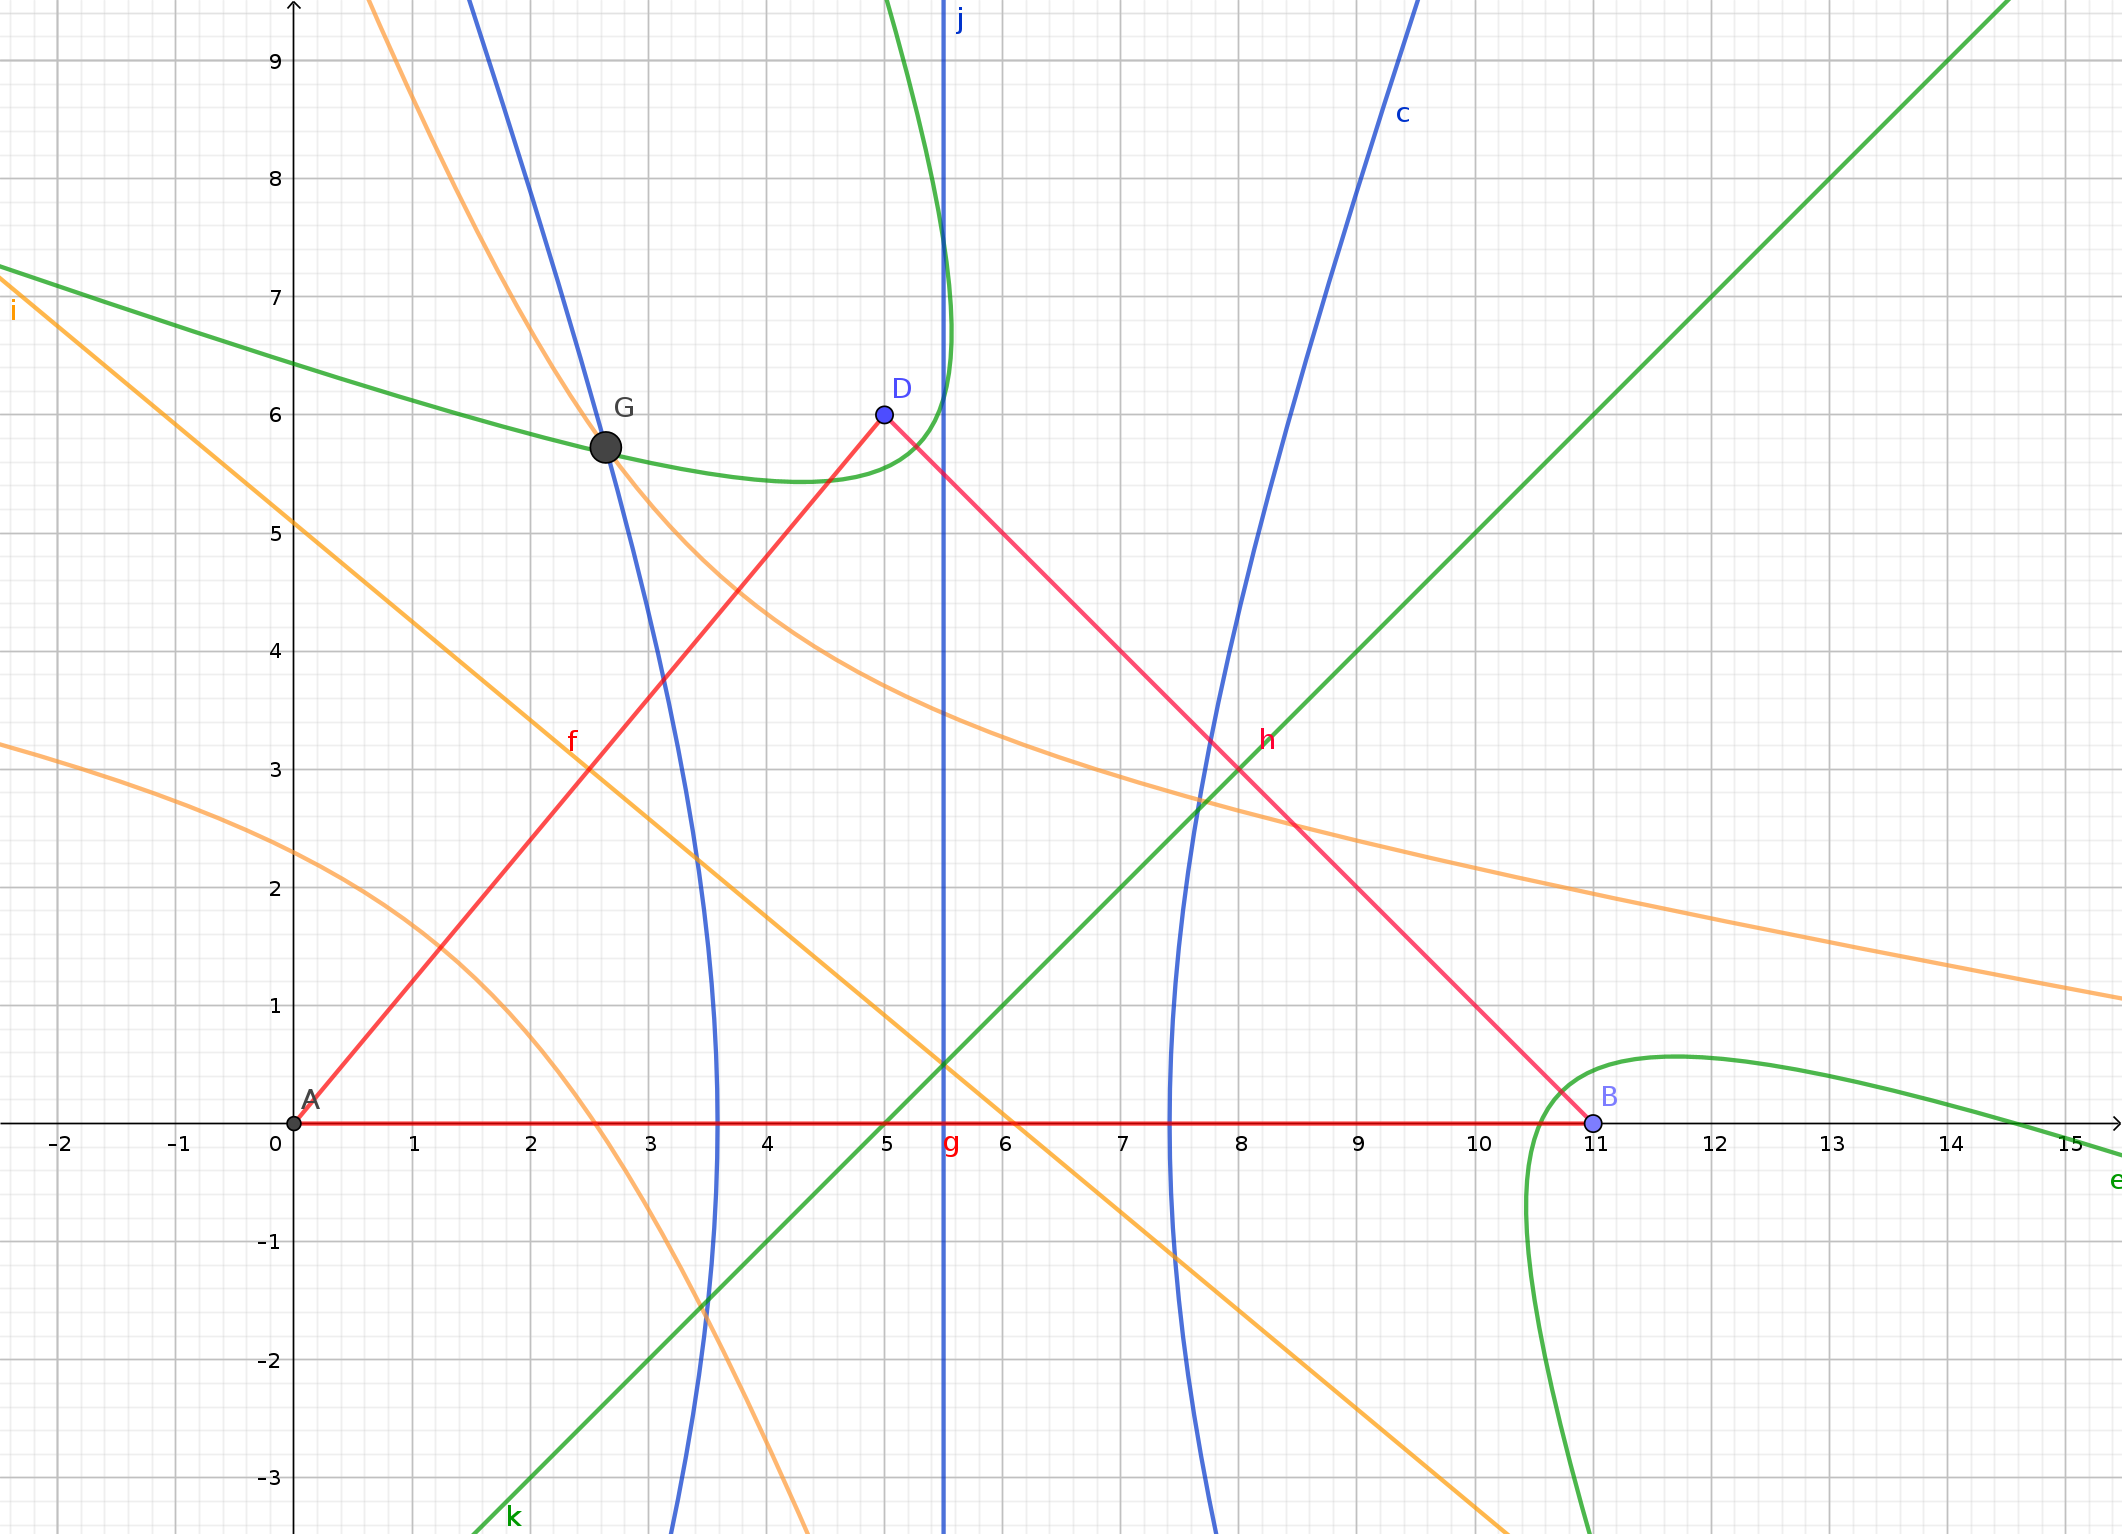
\includegraphics[width=1\textwidth]{tdoa.png}
    \caption{Localization using TDoA}
    \label{fig:tdoa}
\end{figure}

\subsection{Phase Difference of Arrival (PDoA)}
In the PDoA method, devices carry two antennas and measure the phase difference of arrival of the RF signal. Assume two antennas are separated by a distance $d$, with a wavefront incident at an angle $\theta$, then the extra path the signal must travel between antenna 1 and antenna 2 (see figure \ref{fig:PhaseInterferometry}) results in a phase difference, \Delta\Phi, between the two antennas. The incident angle $\theta$ can be calculated using equation \ref{eqn:pdoa_incident_angle}.

\begin{equation}
    \theta = \arcsin(\frac{\lambda\Delta\Phi}{2\pi d})
    \label{eqn:pdoa_incident_angle}
\end{equation}

In 2D Euclidean space, the location of the unknown-location tag is the intersection on two incident line as illustrated in figure \ref{fig:pdoa}.
\begin{figure}[H]
    \centering
    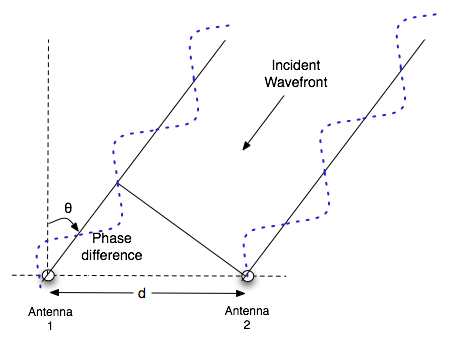
\includegraphics[width=0.5\textwidth]{PhaseInterferometry.png}
    \caption{Phase Difference of Arrival}
    \label{fig:PhaseInterferometry}
\end{figure}

\begin{figure}[H]
    \centering
    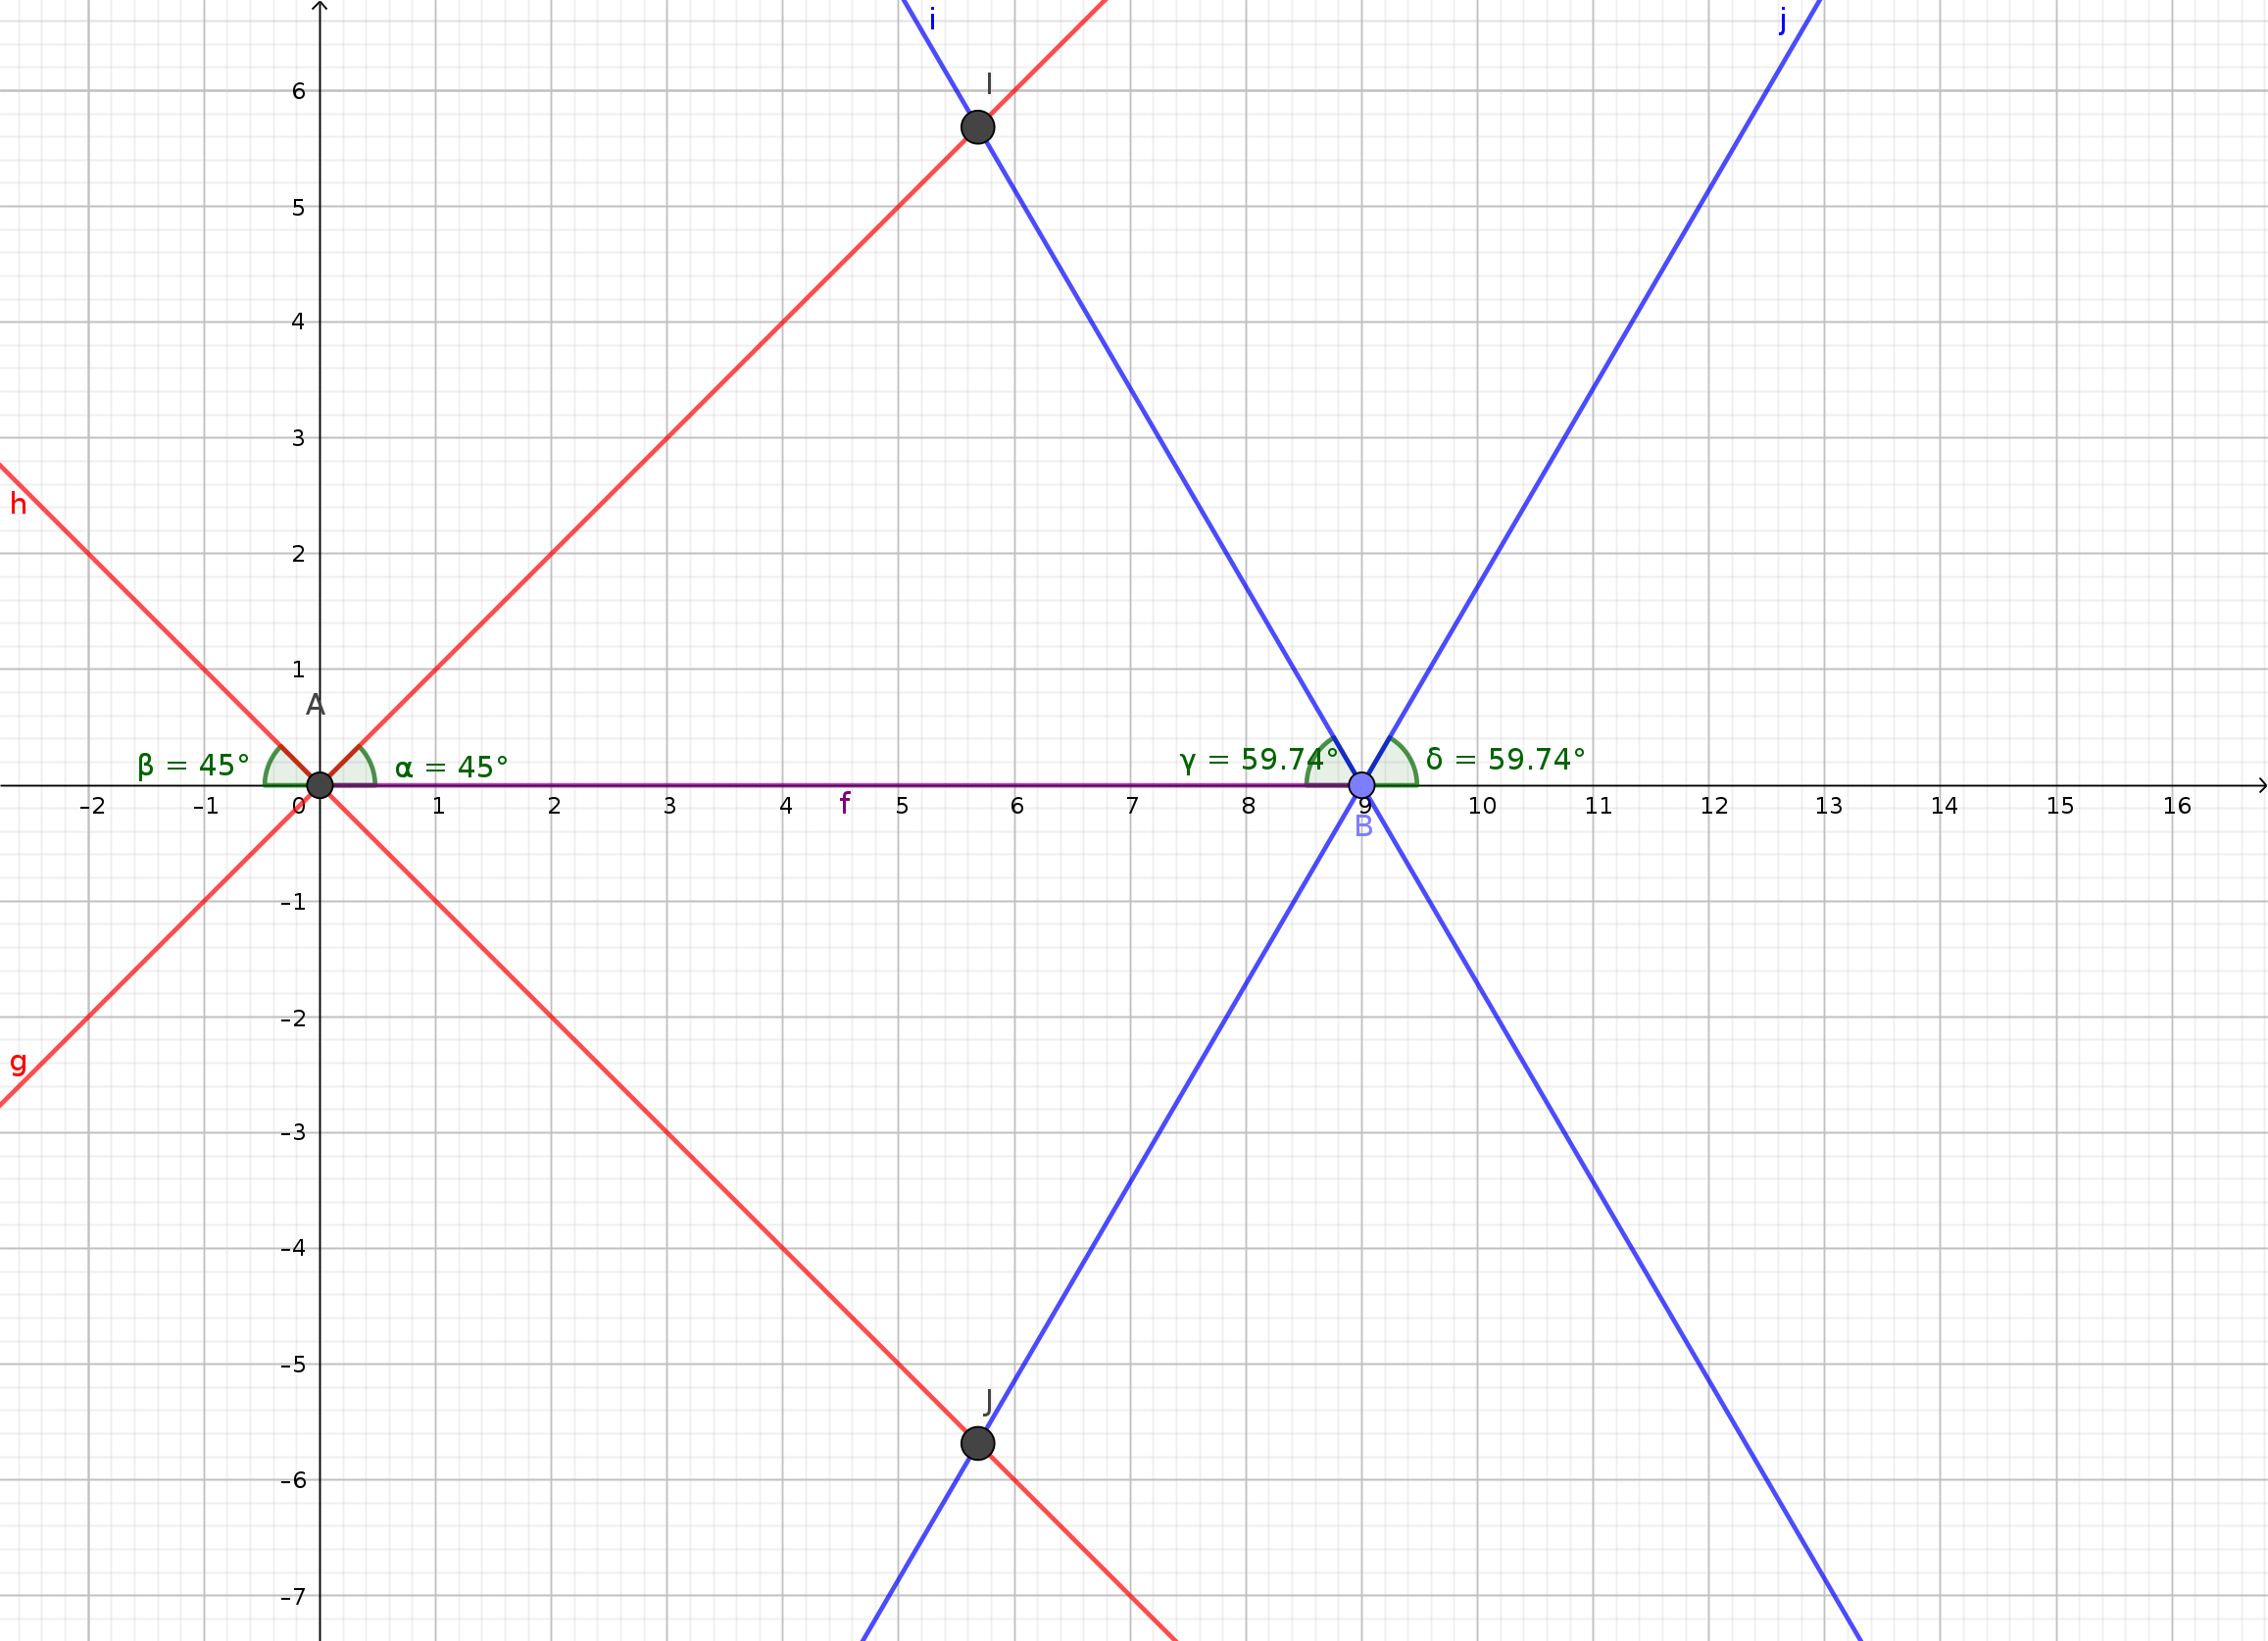
\includegraphics[width=1\textwidth]{pdoa.png}
    \caption{Localization using PDoA}
    \label{fig:pdoa}
\end{figure}

\subsection{Two-Way Ranging (TWR)}
The TWR method relies on two-way communication between devices. As they communicate, the devices also measure the time of flight of the RF signal. The actual distance between the two devices can be derived by multiplying the round trip time of the signal by the speed of light, and then dividing by 2. Equation \ref{eqn:pos_est_twr_tof} is used for the purpose of calculating distance as illustrated in figure \ref{fig:twr_anchor_and_tag}.

\begin{equation}
    tof = \frac{1}{2} ((tt2 - tt1) - (ta2 - ta1))
    \label{eqn:pos_est_twr_tof}
\end{equation}

Applying the TWR scheme between two devices, the distance between them can be measured and utilized to find the location of tags. One simple way to find the position from distances is to solve the intersection between circles, spheres or n-spheres as illustrated in figure \ref{fig:twr_trilateration}.

This thesis uses the TWR approach to obtain distances. The multilateration method utilized to solve the location is described in the following section.

\begin{figure}[H]
    \centering
    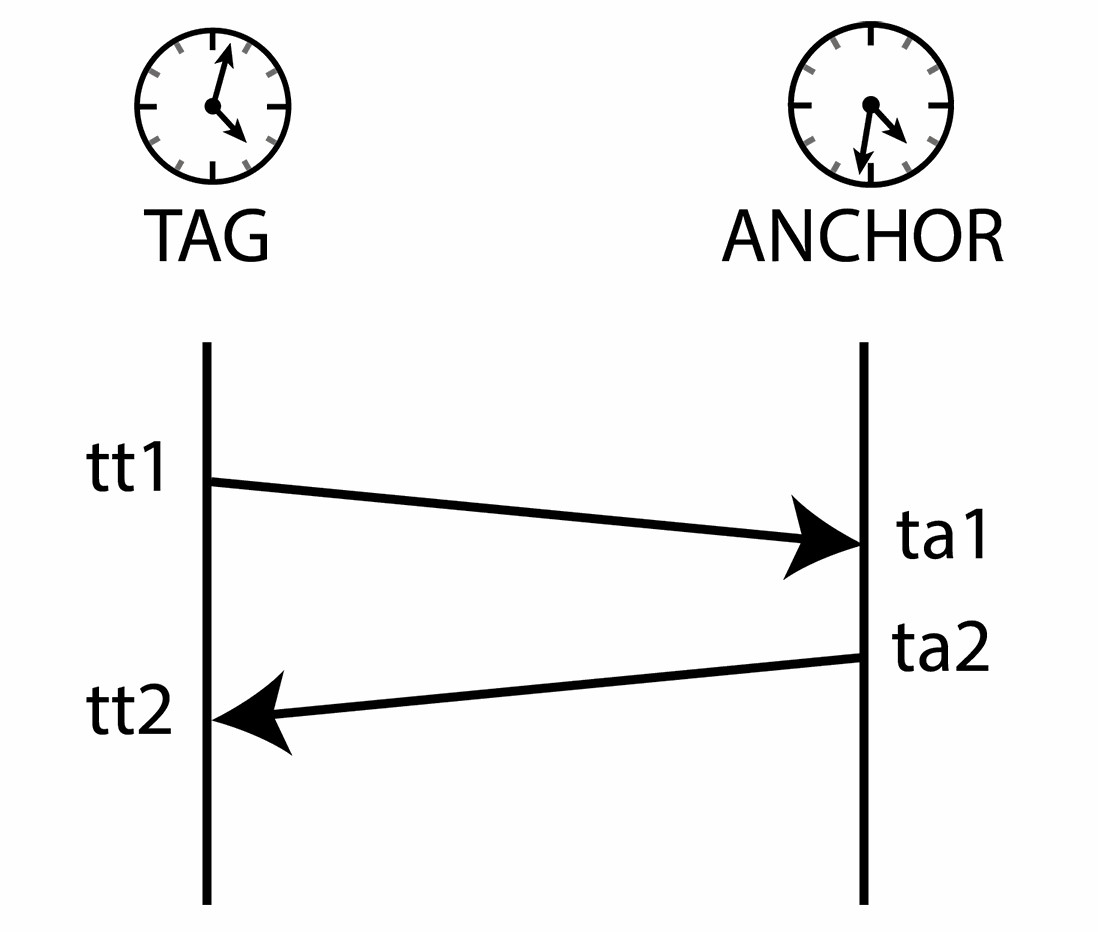
\includegraphics[width=0.4\textwidth]{twr_protocol.png}
    \caption{Two-Way Ranging}
    \label{fig:twr_anchor_and_tag}
\end{figure}

\begin{figure}[H]
    \centering
    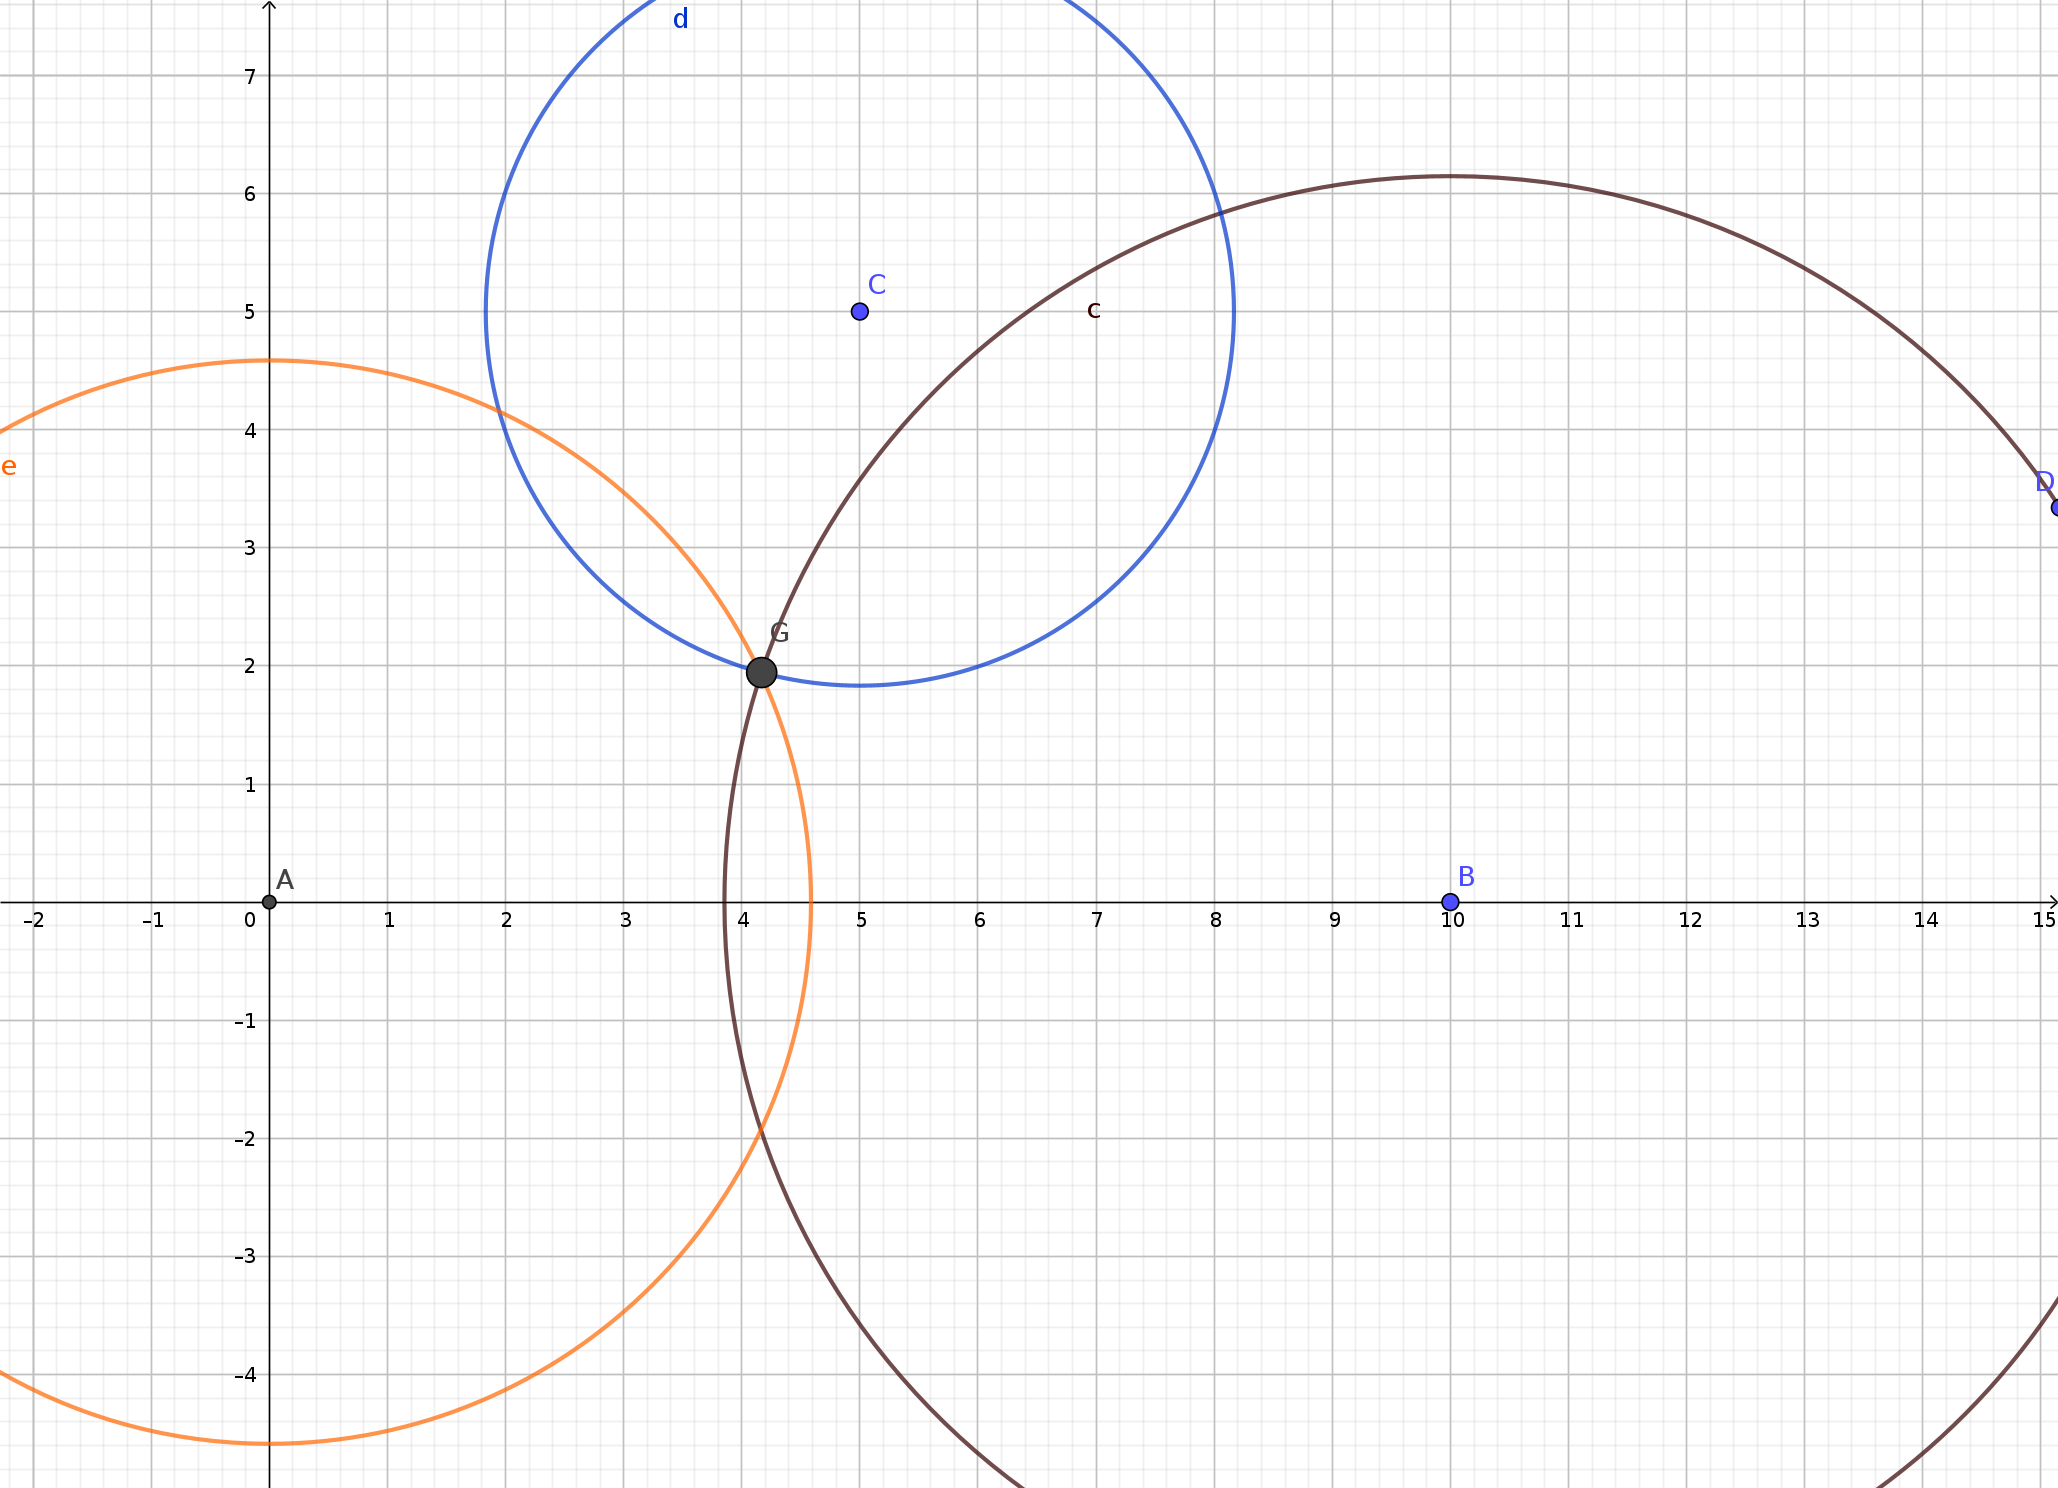
\includegraphics[width=1\textwidth]{twr.png}
    \caption{Localization using TWR}
    \label{fig:twr_trilateration}
\end{figure}

\section{Multilateration in Three-dimensional Euclidean Space}
\label{sec:localization_using_multilateration}

Suppose there are three unique anchor points in three dimensional space: $A_1(x_1, y_1,z_1)$, $A_2(x_2, y_2,z_2)$,
and $A_3(x_3, y_3,z_3)$ and an unknown tag point $T(x,y,z)$ with three known distances to each anchor point:
\begin{equation}
    \begin{split}
        d_1 = | T - A_1| \\
        d_2 = | T - A_2| \\
        d_3 = | T - A_3|
    \end{split}
\end{equation}
The problem of finding the coordinates of $T$ is called multilateration in 3D space. The name is derived from trilateration, a  geometrical problem of determining an unknown position on a plane based on the distance to other two known vertices of a triangle (the length of two sides). In this section, closed-form solution for multilateration problem is derived base on a simplified problem.

\subsection{Simplified Problem}
\label{subsection:multilateration_simplified_problem}
For simplicity, assume that the three anchor points lie on the $xy$ plane with $z = 0$. Rewriting the coordinates of the three anchors: $A_1(0,0,0)$, $A_2(x_2,0,0)$, $A_3(x_3,y_3,0)$ with $x_2 \neq 0$, $x_3 \neq 0$ and $y_3 \neq 0$, then equation of the sphere associated with each anchor is as follows:
\begin{subequations}
    \begin{align}
        A_1 &\Rightarrow  x^2 + y^2 + z^2 = d_1^2 \label{eqn:d1_t_a_a}\\
        A_2 &\Rightarrow (x-x_2)^2 + y^2 + z^2 = d_2^2 \label{eqn:d1_t_a_b}\\
        A_3 &\Rightarrow (x-x_3)^2 + (y-y_3)^2 + z^2 = d_3^2 \label{eqn:d1_t_a_c}
    \end{align}
\end{subequations}
\begin{figure}[H]
    \centering
    \includegraphics[width=0.8\textwidth]{simplified_multilateration.png}
    \caption{Simplified multilateration}
    \label{fig:simplified_multilateration}
\end{figure}
Subtract equations \ref{eqn:d1_t_a_b} and \ref{eqn:d1_t_a_a} to solve for $x$:
\begin{equation}
    \begin{split}
        x_2^2 - 2x_2x + x^2 + y^2 + z^2 &= d_2^2\\
        x^2 + y^2 + z^2 &= d_1^2 \\
        \cline{1-2}
        x_2^2 - 2x_2x &= d_2^2 - d_1^2 \\
        \Leftrightarrow 2xx_2 &=  d_1^2 - d_2^2 + x_2^2 \\
        \Leftrightarrow x &= \frac{d_1^2 - d_2^2 + x_2^2}{2x_2}
    \end{split}
    \label{eqn:simplified_multilateration_x}
\end{equation}
Subtract equations \ref{eqn:d1_t_a_c} and \ref{eqn:d1_t_a_a} to solve for $y$:
\begin{equation}
    \begin{split}
        x_3^2  - 2x_3x + y_3^2 - 2y_3y + x^2 + y^2 + z^2 &= d_3^2 \\
        x^2 + y^2 + z^2 &= d_1^2 \\
        \cline{1-2}
        x_3^2  - 2x_3x + y_3^2 - 2y_3y &= d_3^2 - d_1^2\\
        \Leftrightarrow 2y_3y &= d_1^2 - d_3^2 + x_3^2 + y_3^2 - 2x_3x \\
        \Leftrightarrow y &= \frac{d_1^2 - d_3^2 + x_3^2 + y_3^2 - 2x_3x}{2y_3} \\
        &= \frac{d_1^2 - d_3^2 + x_3^2 + y_3^2 - \frac{x_3(d_1^2 - d_2^2 + x_2^2)}{x_2}}{2y_3}
    \end{split}
    \label{eqn:simplified_multilateration_y}
\end{equation}
Plug \ref{eqn:simplified_multilateration_x} and \ref{eqn:simplified_multilateration_y} into \ref{eqn:d1_t_a_a} for solving $z$:
\begin{equation}
    \begin{split}
        z &= \pm \sqrt{d_1^2 - x^2 - y^2} \\
        &= \pm \sqrt{d_1^2 - \left(\frac{d_1^2 - d_2^2 + x_2^2}{2x_2}\right)^2 - \left(\frac{d_1^2 - d_3^2 + x_3^2 + y_3^2 - \frac{x_3(d_1^2 - d_2^2 + x_2^2)}{x_2}}{2y_3}\right)^2}
    \end{split}
    \label{eqn:simplified_multilateration_z}
\end{equation}
There are unique solutions to the simplified multilateration problem, since the result of three intersecting spheres are two points.

\subsection{A Closed-form Solution for Multilateration Problem}
To fully solve the multilateration problem in Euclidean space, $A_1$, $A_2$, $A_3$ is firstly transformed to the coordinate as the above simplified problem. Since the distances are invariant under such transformation which are the linear and rotation transformation, $T$ can be found using \ref{eqn:simplified_multilateration_x}, \ref{eqn:simplified_multilateration_y} and \ref{eqn:simplified_multilateration_z}. $T$ is then transformed to the original coordinate to get the final result.

Let $S =\{\boldsymbol{e_x}, \boldsymbol{e_y}, \boldsymbol{e_z}\}$ is the basis of the new vector space. Then $A_1$, $A_2$, $A_3$ can be written uniquely as a linear combination of vectors in the basis $S$. Basis $S$ is specially chosen to make the general problem become the simplified problem. As shown in equation \ref{eqn:multilateration_ex}, $\boldsymbol{e_x}$ is a unit vector lies on $\overrightarrow{A_1A_2}$.

\begin{equation}
    \boldsymbol{e_x} = \frac{A_2-A_1}{\Vert A_2 - A_1\Vert}
    \label{eqn:multilateration_ex}
\end{equation}

Since $\Vert \boldsymbol{e_x} \Vert = 1$, the scalar projection of $\overrightarrow{A_1A_3}$ onto $\overrightarrow{A_1A_2}$ is:
\begin{equation}
    \begin{split}
    V_x &= \Vert A_3 - A_1 \Vert \cos{\gamma} \\
    &= \Vert \boldsymbol{e_x} \Vert \Vert A_3 - A_1 \Vert \cos{\gamma}\\
    &= \boldsymbol{e_x} \cdot (A_3 - A_1)      
    \end{split}
\end{equation}

\begin{figure}[H]
    \centering
    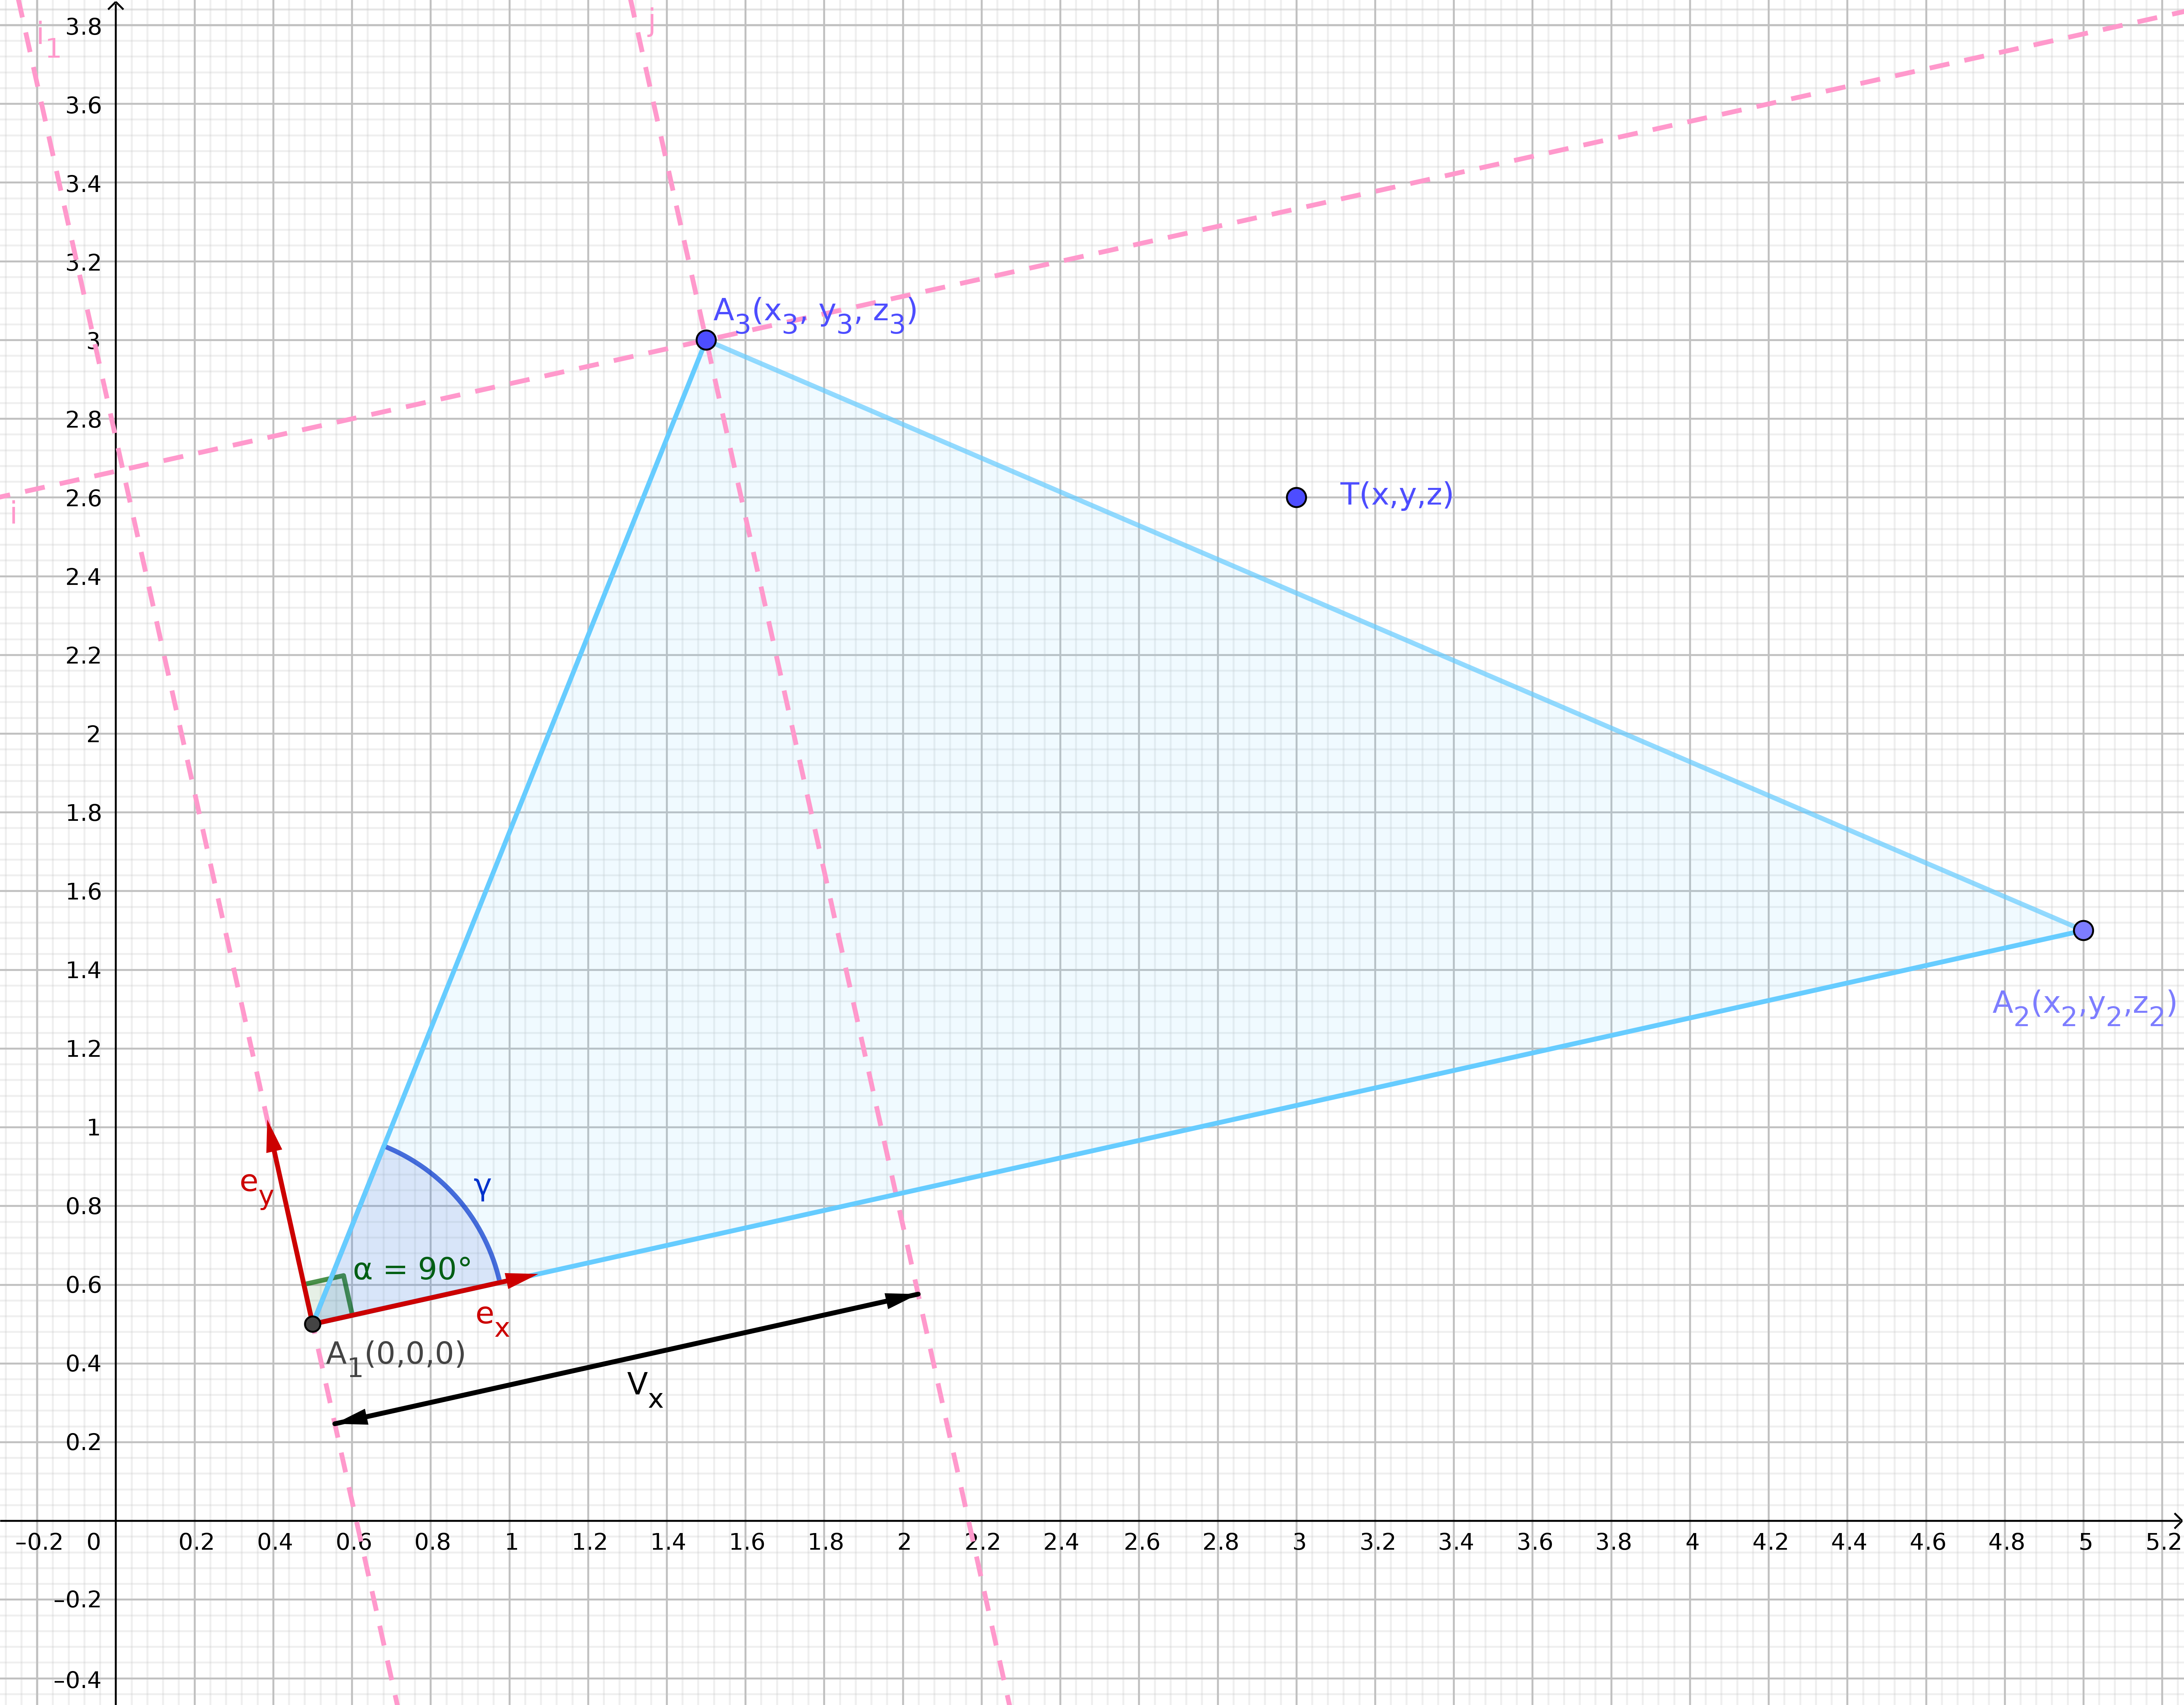
\includegraphics[width=0.9\textwidth]{multilateration.png}
    \caption{Multilateration in Euclidean space}
    \label{fig:multilateration}
\end{figure}

The component of $\overrightarrow{A_1A_3}$ lies on $e_y$ is $A_3-A_1-(s*\boldsymbol{e_x})$. Hence:
\begin{equation}
    \boldsymbol{e_y} = \frac{A_3-A_1-(s*\boldsymbol{e_x})}{\Vert A_3-A_1-(s*\boldsymbol{e_x})\Vert}
\end{equation}
Finally, $\boldsymbol{e_z}$ is the cross product of the two other unit vectors.
\begin{equation}
    \boldsymbol{e_z} = \boldsymbol{e_x} \times \boldsymbol{e_y}
\end{equation}

In the basis $S$, the new set of points is:
\begin{equation}
    \begin{split}
        &B_0(0,0,0) \\
        &B_1(U, 0, 0) = B_1(\Vert A_2 - A_1 \Vert, 0, 0) \\
        &B_2(V_x, V_y, 0) = B_2(\boldsymbol{e_x} \cdot (A_3 - A_1), \boldsymbol{e_y} \cdot (A_3 - A_1), 0) 
    \end{split}
    \label{eqn:multilateration_to_simplified_problem}
\end{equation}
As the distance is invariant to basis change, the coordinates of $T$ in the $S$ basis can be found using \ref{eqn:multilateration_to_simplified_problem} as described in section \ref{subsection:multilateration_simplified_problem}.

Suppose that the coordinates of $T$ found in the basis $S$ are $T'_1(x_t,y_t,z_t)$ and $T'_2(x_t, y_t, -z_t)$, the coordinates of $T$ in the original coordinate can calculated using equation \ref{eqn:multilateration_inverse_transfrom}.
\begin{equation}
    \begin{split}
        T_1 = A_1 + x_t\boldsymbol{e_x} + y_t\boldsymbol{e_y} + z_t\boldsymbol{e_z} \\
        T_2 = A_1 + x_t\boldsymbol{e_x} + y_t\boldsymbol{e_y} - z_t\boldsymbol{e_z} 
    \end{split}
    \label{eqn:multilateration_inverse_transfrom}
\end{equation}

\subsection{Multilateration Implementation}

In a real scenario, distances to other known points are used for selecting the final location from the two locations. The chosen location should have a distance to the known point being closest to the given one. If multiple distances are available, voting may be one solution.

A python implementation for multilateration in Euclidean space is shown in figure \ref{fig:multilateration_python_implementation}.

With the C struct given in figure \ref{fig:c_struct_for_multilateration}, a C implementation for multilateration in Euclidean space is provided in figure \ref{fig:multilateration_c_implementation}. In this thesis, the C implementation is used by the tag to solve its location itself from distances to anchors.

\begin{figure}[H]
    \begin{python}
import numpy as np

def multilateration(distances):
    A1=np.array(distances[0][:3])
    A2=np.array(distances[1][:3])
    A3=np.array(distances[2][:3])
    d1=distances[0][-1]
    d2=distances[1][-1]
    d3=distances[2][-1]

    U=np.linalg.norm(A2-A1)
    e_x=(A2-A1)/U
    Vx=np.dot(e_x,(A3-A1))
    e_y=(A3-A1-(Vx*e_x))/(np.linalg.norm(A3-A1-(Vx*e_x)))
    Vy=np.dot(e_y,(A3-A1))
    e_z=np.cross(e_x,e_y)

    x=(d1**2-d2**2+U**2)/(2*U)
    y=(d1**2-d3**2+Vx**2+Vy**2-2*Vx*x)/(2*Vy)
    z1=np.sqrt(d1**2-x**2-y**2)
    z2=-z1

    T1=A1+(x*e_x)+(y*e_y)+(z1*e_z)
    T2=A1+(x*e_x)+(y*e_y)+(z2*e_z)
    return T1, T2
    \end{python}
    \caption{Python implementation for multilateration in Euclidean space}
    \label{fig:multilateration_python_implementation}
\end{figure}

\begin{figure}[H]
    \begin{lstlisting}[style=CStyle]
typedef struct sphere
{
    float x;
    float y;
    float z;
    float r;
}sphere_t;

typedef struct location
{
    float x;
    float y;
    float z;
}location_t;

typedef struct trilateration_result{
    location_t PA;
    location_t PB;
}trilateration_result_t;
\end{lstlisting}
\caption{C struct for multilateration}
\label{fig:c_struct_for_multilateration}
\end{figure}

\begin{figure}[H]
    \begin{lstlisting}[style=CStyle]
void trilaterate(sphere_t sphere[3], trilateration_result_t *trilateration_result){
    /* Prepare all parameters */
    float a0x = sphere[0].x;
    float a0y = sphere[0].y;
    float a0z = sphere[0].z;
    float a1x = sphere[1].x;
    float a1y = sphere[1].y;
    float a1z = sphere[1].z;
    float a2x = sphere[2].x;
    float a2y = sphere[2].y;
    float a2z = sphere[2].z;
    float r0 = sphere[0].r;
    float r1 = sphere[1].r;
    float r2 = sphere[2].r;

    /* Transform to new coordinate system */
    float a1tx = a1x - a0x;
    float a1ty = a1y - a0y;
    float a1tz = a1z - a0z;
    float a2tx = a2x - a0x;
    float a2ty = a2y - a0y;
    float a2tz = a2z - a0z;
    
    float U = sqrt(a1tx*a1tx + a1ty*a1ty + a1tz*a1tz);
    float exx = a1tx/U;
    float exy = a1ty/U;
    float exz = a1tz/U;
    float Vx = a2tx*exx + a2ty*exy + a2tz*exz;
    float temp_x = a2tx - Vx*exx;
    float temp_y = a2ty - Vx*exy;
    float temp_z = a2tz - Vx*exz;
    float Vy = sqrt(temp_x*temp_x + temp_y*temp_y + temp_z*temp_z);
    float eyx = temp_x/Vy;
    float eyy = temp_y/Vy;
    float eyz = temp_z/Vy;
    float ezx = exy*eyz - exz*eyy;
    float ezy = exz*eyx - exx*eyz;
    float ezz = exx*eyy - exy*eyx;

    /* Trilateration */
    float x  = (r0*r0 - r1*r1 + U*U) / (2*U);
    float y  = (r0*r0 - r2*r2 + Vx*Vx + Vy*Vy - 2*Vx*x) / (2*Vy);
    float z  = r0*r0 - x*x - y*y;
    if(z < 0) z = 0;
    float z0 = sqrt(z);
    float z1 = -z0;

    /* Transform to original coordinate system */
    trilateration_result->PA.x = a0x + x*exx + y*eyx + z0*ezx;
    trilateration_result->PA.y = a0y + x*exy + y*eyy + z0*ezy;
    trilateration_result->PA.z = a0z + x*exz + y*eyz + z0*ezz;

    trilateration_result->PB.x = a0x + x*exx + y*eyx + z1*ezx;
    trilateration_result->PB.y = a0y + x*exy + y*eyy + z1*ezy;
    trilateration_result->PB.z = a0z + x*exz + y*eyz + z1*ezz;
}
    \end{lstlisting}
    \caption{C implementation for multilateration in Euclidean space}
    \label{fig:multilateration_c_implementation}
\end{figure}

\section{ToF to Distance}
The result obtained from TWR method is the time of a flight between anchor and tag. However, the required distance needs to be measured in meters. A linear regression model is good enough to estimate the relationship between ToF and the actual distance as illustrated in figure \ref{fig:tof_to_distance}.
\begin{figure}[H]
    \begin{center}
        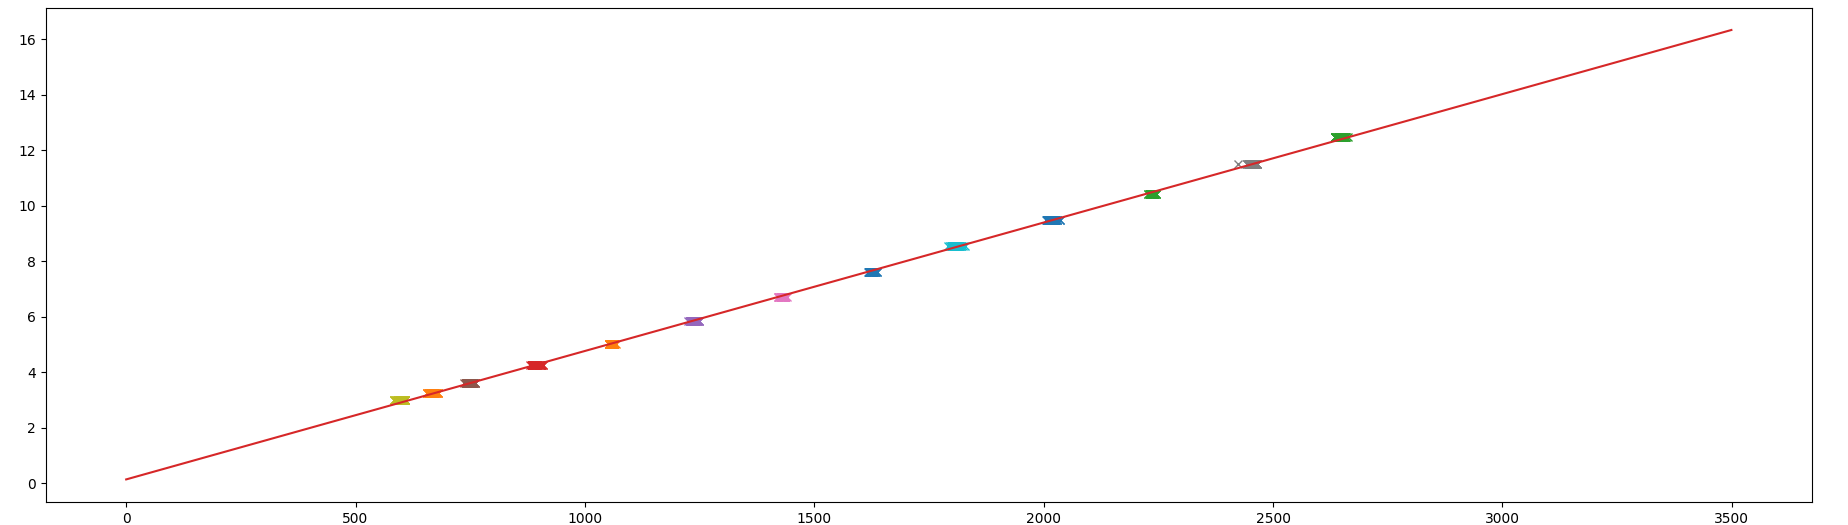
\includegraphics[width=1\textwidth]{tof_to_distance.png}
    \end{center}
    \caption{ToF to distance}
    \label{fig:tof_to_distance}
\end{figure}
The LinearRegression model of sklearn library is utilized to approximate the distance based on ToF. The result is shown in equation \ref{eqn:distance_model}.
\begin{equation}
    d = w*ToF + b
    \label{eqn:distance_model}
\end{equation}
Where:
\begin{itemize}
    \item $d$: The distance between tag and anchor
    \item $ToF$: The time of a flight between tag and anchor
    \item $w = 0.004632130984819555$: The slope of estimated model 
    \item $b = 0.13043560944811894$: The bias of estimated model
\end{itemize}

Loss function of the linear model is given in equation \ref{eqn:distance_model_loss}.
\begin{equation}
    e = \frac{1}{n} \sum_{k = 1}^{n} | d^k_{est}-d^k \vert = \frac{1}{n} \sum_{k = 1}^{n} | w*ToF^k + b -d^k \vert  = 0.04095793575440317 (m)
    \label{eqn:distance_model_loss}
\end{equation}
Where:
\begin{itemize}
    \item $d^k_{est}$ is the $k$th estimated distance
    \item $d^k$ is the $k$th reference distance
\end{itemize}

In an ideal scenario, the mean error of the linear model is less than 5cm.

\end{document}